\documentclass{article}
\usepackage{listings}
\usepackage{dirtytalk}
\usepackage{amssymb,amsmath}
\usepackage{minted}
\usepackage{hyperref}
\usepackage{graphicx}

\graphicspath{ {images/} }

\begin{document}

\title{Indoor Localisation, Localisation Algorithm}
\author{Sebastian Hojas, 014570704}

\maketitle

\section{Instructions}

The program that computes the location is a Python (2.7) script and takes the following arguments:

\begin{verbatim}
  Usage: python2.7 Localiser.py <input_file> [<database>]
         Input file is required, database optional.
\end{verbatim}

\section{Test results}

\begin{verbatim}
  python2.7 Localiser.py test.fingerprints train.fingerprints

  >  x= 2  y= 2089  z= 474
\end{verbatim}

\section{Algorithm}

\begin{enumerate}
  \item Find n best matches
    \subitem Missing matches are penalised with a small factor
    \subitem On the other hand, intersecting coverage is being rewarded exponentially
  \item Calculate average point based on all matches
  \item Remove n/2 points furthest away from the average point (medianisation)
  \item Calculate weighted average of points
\end{enumerate}

I have been testing different values of n and went with $n=10$ in the end.

\section{Database format}

I wanted to formly specifiy the fingerprints in \textit{scans/db.fingerprints}. Each line represents one fingerprint and has the following format:

\begin{verbatim}
  x;y;z;[MAC;RSSI]
    [] .. represents revision (no brackets used in the actual file)
\end{verbatim}

\section{Taking fingerprints}

I have been taking fingerprints dynamically by walking from point to point and distributing it by timestamp.
I have collected roughly 240 prints. One problem I have encountered is that my scans on OSX vary significantly. The closest matches are often somewhere completely different. I could not yet validate whether my algorithm supports this behaviour or the measurements vary so significantly. 
I have tried to work around this by removing potential matches far away from the average point in the matching algorithm.

\begin{figure}[h]
  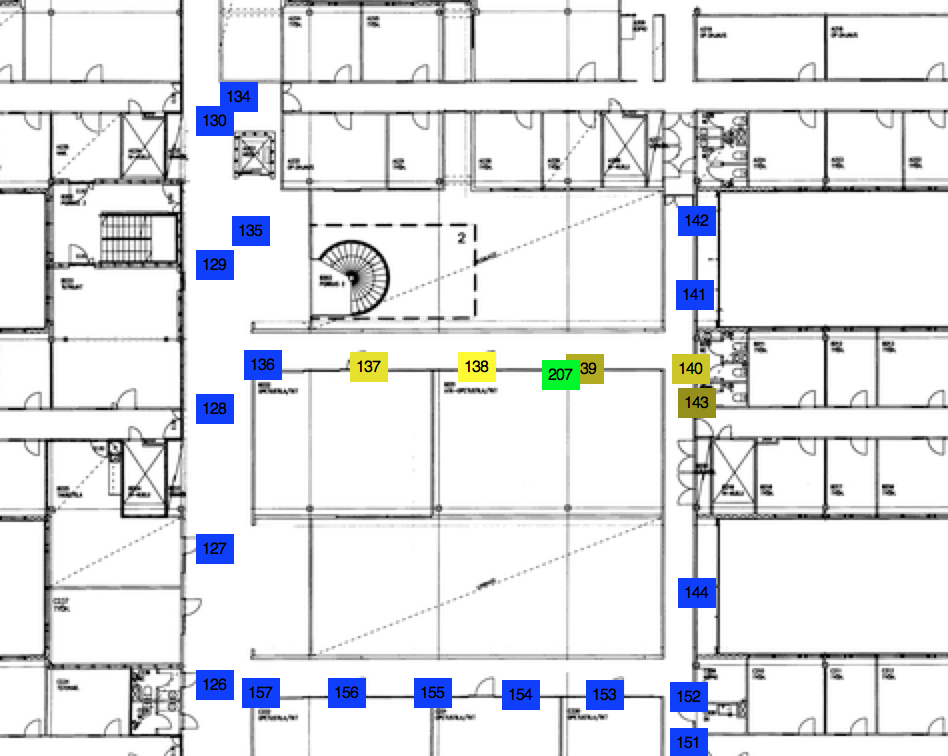
\includegraphics[scale=0.7]{prototype}
  \caption{Prototype visualising measurements and localisation result. The green points represent the estiamted location. Blue points represent the non-matched fingerprints. Yellow-shaded fingerprints represent matched fingerprints (bright yellow = strong matching, dark yellow = weak matching)}
\end{figure}

\end{document}



